\documentclass[12pt]{article}

% Language setting
% Replace `english' with e.g. `spanish' to change the document language
\usepackage[spanish]{babel}

% Set page size and margins
% Replace `letterpaper' with`a4paper' for UK/EU standard size
\usepackage[a4paper,top=2cm,left=3cm,right=1.5cm,marginparwidth=1.75cm]{geometry}

% Useful packages
\usepackage{amsmath}
\usepackage{xcolor}
\usepackage{graphicx}
\usepackage[font=footnotesize,labelfont=bf]{caption}
\usepackage[allbordercolors=orange]{hyperref}
\usepackage{fontspec}
\usepackage{fancyhdr}
\usepackage{titling}
\usepackage{array}
\usepackage{multicol}
\usepackage{framed}
\usepackage{enumitem}
\usepackage[bibstyle=numeric, citestyle=numeric, sorting=nyt]{biblatex}
\usepackage{soul}
\usepackage{subcaption}
\usepackage{wrapfig}
\usepackage{listings}
\usepackage{layout}

\addbibresource{TIPPRA1.bib}

\definecolor{uocblue}{HTML}{000078}
\colorlet{main}{uocblue}
\setmainfont{Arial}[Color = uocblue]
\renewcommand{\labelitemi}{$\textcolor{uocblue}{\bullet}$}
\renewcommand{\labelitemii}{$\textcolor{uocblue}{\cdot}$}
\renewcommand{\labelitemiii}{$\textcolor{uocblue}{\diamond}$}
\renewcommand{\labelitemiv}{$\textcolor{uocblue}{\ast}$}
\renewcommand{\thefootnote}{\textbf{\arabic{footnote}}}
\renewcommand{\footnoterule}{{
		\color{uocblue}
		\kern 20pt
		\hrule width 2in
		\kern 3pt
}}
\setulcolor{uocblue}

\setcounter{biburllcpenalty}{7000}
\setcounter{biburlucpenalty}{8000}

\hypersetup{allcolors=uocblue}
\urlstyle{same}

% metadata
%%%%%%%%%%%%%%
\newcommand{\master}{Máster en Ciencia de Datos}
\newcommand{\grade}{2021/2022}
\newcommand{\subject}{Tipología y ciclo de vida del dato}
\newcommand{\testname}{\textbf{PRA1}}
\newcommand{\loginuocone}{agomezvarela@uoc.edu}
\newcommand{\loginuoctwo}{plazarotello@uoc.edu}
\newcommand{\authorone}{Alba Gómez Varela}
\newcommand{\authortwo}{Patricia Lázaro Tello}
\title{\textit{Web scraping} del mercado inmobiliario}
\author{Alba Gómez Varela\\Patricia Lázaro Tello}
\date{}	% quitar la fecha del titulo
%%%%%%%%%%%%%%

\pretitle{\vspace{-2cm}\begin{center}\LARGE \bfseries}
	\posttitle{\end{center}}
\preauthor{\vspace{-0.65cm}\begin{center}
		\large \itshape
		\begin{tabular}[t]{c}}
		\postauthor{\end{tabular}\end{center}\vspace{-1.5cm}}


\fancypagestyle{uoc}{
	\fancyhf{}
	\fancyhead[C]{
\includegraphics[width=16.5cm]{uoc.png}}
	\fancyhead[R]{\footnotesize \hspace*{\fill}\authorone \space \space · \space \nolinkurl{\loginuocone}\\
		\hspace*{\fill}\authortwo \space \space \space · \space\space\space \nolinkurl{\loginuoctwo}\\ \vspace{-2pt}}
	\fancyfoot[R]{\footnotesize \thepage} %\hspace{0.5cm}}
\fancyfoot[C]{\footnotesize \hspace{1.5cm} \grade}
\fancyfoot[L]{\footnotesize \subject \space · \testname\\
	\space\master}
\renewcommand{\headrulewidth}{0pt} % remove lines as well
\renewcommand{\footrulewidth}{0pt}
\setlength{\footskip}{50pt}%
\setlength{\headsep}{15pt}
\setlength{\headheight}{42pt}
\setlength{\parskip}{10pt}
\setlength{\topmargin}{-1cm}
%\setlength{\textheight}{\textheight}
\setlength{\textheight}{650pt}
\setlength{\oddsidemargin}{0pt}
\setlength{\marginparsep}{0pt}
\setlength{\marginparpush}{0pt}
\setlength{\voffset}{-10pt}
\setlength{\fboxsep}{0pt}
}

\pagestyle{uoc}
\linespread{1.125}
\color{uocblue}

\newlength{\leftbarwidth}
\setlength{\leftbarwidth}{0.15em}
\newlength{\leftbarsep}
\setlength{\leftbarsep}{0pt}
\renewenvironment{leftbar}{%
\def\FrameCommand{{\vrule width \leftbarwidth\relax\hspace {\leftbarsep}}}%
\MakeFramed {\advance \hsize -\width \FrameRestore }%
}{%
\endMakeFramed
}

\newenvironment{blockquote}{%
\par%
\leftskip=2em
%	\begin{leftbar}
	\noindent\ignorespaces}{%
	%	\end{leftbar}
\par}

\setlength{\parindent}{0em}

%%%%%%%%%%%
\definecolor{codegreen}{rgb}{0,0.6,0}
\definecolor{codegray}{rgb}{0.5,0.5,0.5}
\definecolor{codepurple}{rgb}{0.58,0,0.82}
\definecolor{backcolour}{rgb}{0.97,0.97,0.95}

\lstdefinestyle{mystyle}{backgroundcolor=\color{backcolour}, commentstyle=\color{codegreen},
keywordstyle=\color{magenta}, numberstyle=\tiny\color{codegray}, stringstyle=\color{codepurple},
basicstyle=\ttfamily\footnotesize, breakatwhitespace=false, breaklines=true, captionpos=t,                    
keepspaces=true, numbers=left, numbersep=5pt, showspaces=false,	showstringspaces=false,
showtabs=false, tabsize=4}

\lstset{style=mystyle}

\renewcommand*{\lstlistingname}{Documento}
%%%%%%%%%%%

\begin{document}

%\layout*

\maketitle
\thispagestyle{uoc}

%\vspace{-2em}
\begin{framed}
	\textbf{\underline{Houses for sale in the Salamanca and Villaverde district of Madrid in April 2022}}
	\begin{multicols}{2}
		\begin{itemize}[topsep=0cm,partopsep=0cm,label={},wide]
			\item \textbf{Licencia}: CC BY-NC-SA 4.0
			\item \textbf{Número de campos}: 16
			\item \textbf{Número de registros}: 3.545
			\columnbreak
			\item \textbf{DOI}: \href{https://doi.org/10.5281/zenodo.6423459}{10.5281/zenodo.6418974}
			\item \textbf{Fecha de extracción}: primera semana de abril de 2022
		\end{itemize}
	\end{multicols}
\end{framed}

\vspace{-2em}

\section{Contexto}\label{contexto}\vspace{-1.0em}

La \textbf{Ley por el Derecho a la Vivienda} se aprobó en España por decreto el 1 de febrero de 2022 y, aunque esta normativa no regula los pisos en venta ya construidos en la actualidad de forma directa, sí que podría afectar a su precio en el futuro. Por ejemplo, si se limita el precio del alquiler, se puede dar el caso de que los inversores dejen de estar interesados en estos bienes y por tanto, el precio final de venta variaría al cambiar la demanda. Por otro lado, el 30\% de las nuevas promociones se reservará a Viviendas de Protección Oficial (VPO), lo que también puede alterar el precio de la vivienda libre.

Además de cambios en la normativa del mercado inmobiliario, la \textbf{invasión de Rusia a Ucrania} ha pillado por sorpresa a todos los sectores de la economía, disparando la \textbf{inflación} en España hasta un 9,8\%, según indicador adelantado del IPC para el mes de marzo publicado por el Instituto Nacional de Estadística (INE). Del mismo modo, el Banco de España ha recortado sus \textbf{previsiones de crecimiento} para el país y ha doblado su previsión anual de inflación al 7,5\%, según los datos publicados el 5 de abril de 2022.

Asimismo, cabe destacar que el mercado inmobiliario en España se ha caracterizado desde hace décadas por las \textbf{diferencias en el precio} de la vivienda, tanto según las zonas del territorio nacional como dentro de las propias localidades. 

Teniendo presente esta situación de cambios económicos y normativos, y no existiendo un registro público de viviendas en venta actualizado, se ha decidido obtener la información de las viviendas en venta de los portales inmobiliarios de \textbf{Idealista} y \textbf{Fotocasa}. Esta decisión se fundamenta en que son los portales \textbf{más visitados} en España, según los datos de febrero de \href{https://www.similarweb.com/top-websites/spain/category/business-and-consumer-services/real-estate/}{\textit{similarweb}}, que publica las métricas oficiales de los sitios web de todo el mundo. Además, esta clasificación de visitas se mantiene en los últimos años, por lo que no se prevé que varíe en un corto periodo de tiempo. Asimismo, es interesante que estos portales trabajan tanto con \textbf{inmobiliarias} como con \textbf{particulares} que desean vender inmuebles, por lo que proporcionan una información amplia sobre el tema de interés del proyecto.

\vspace{-1.5em}\section{Houses for sale in the Salamanca and Villaverde district of Madrid in April 2022}\vspace{-1.0em}

Debido a la gran cantidad de conjuntos de datos existentes sobre la temática seleccionada, para el \textit{dataset} resultante se ha optado por un título \textbf{muy descriptivo} a la par que \textbf{concreto}, de modo que solo con él se pueda saber el contenido del mismo. Además, debido a la volatilidad del mercado inmobiliario, se ha decidido incluir el mes de extracción de los datos.

\vspace{-1.5em}\section{Descripción del \textit{dataset}}\vspace{-1.0em}

El conjunto de datos obtenido a partir de los \textit{scrapers} hace referencia a todos los pisos disponibles durante la primera semana de abril de 2022 para su compra en los distritos de Villaverde y Salamanca en la ciudad de Madrid en los sitios web de Idealista y Fotocasa.

Se trata por tanto de una \textit{snapshot} del mercado inmobiliario en el distrito con el precio/m\textsuperscript{2} más bajo (Villaverde) y más alto (Salamanca) en Madrid. Con esta selección de distritos se busca descubrir las características que poseen los pisos de cada distrito, y si existe alguna otra razón, además del distrito en que se encuentra cada vivienda, que justifique su precio.

\vspace{-1.5em}\section{Representación gráfica}\vspace{-1.0em}

Dibujar un esquema o diagrama que identifique el
dataset visualmente y el proyecto elegido

\vspace{-1.5em}\section{Contenido}\vspace{-1.0em}

Explicar los campos que incluye el dataset, el periodo de tiempo de los datos y cómo se han recogido

Los datos han sido obtenidos durante la primera semana de abril de 2022 (del 4 al 10 de abril) de los portales inmobiliarios Idealista y Fotocasa. Los registros obtenidos representan la mayor parte de las viviendas en venta en los distritos Villaverde y Salamanca en la ciudad de Madrid.

\begin{figure}[h]
	\centering
	\captionsetup{font={normalsize}}
	\caption{Distritos de Villaverde y Salamanca \textit{scrapeados}}
	\begin{subfigure}{0.5\textwidth}
		\centering
		\fbox{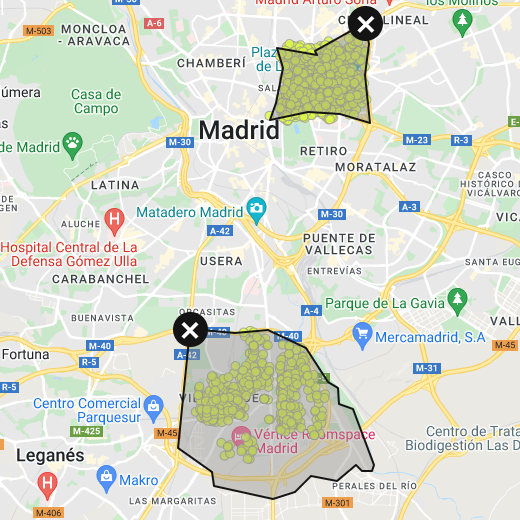
\includegraphics[width=\linewidth]{idealista-villaverde-salamanca}}
		\caption{\vspace{1.5em}Idealista}
	\end{subfigure}%
	\begin{subfigure}{0.5\textwidth}
		\centering
		\fbox{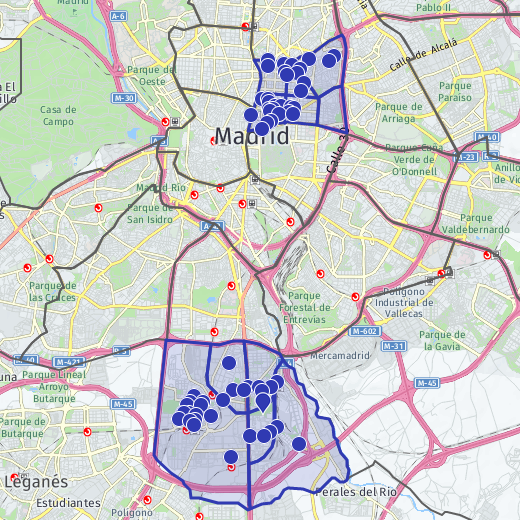
\includegraphics[width=\linewidth]{fotocasa-villaverde-salamanca}}
		\caption{\vspace{1.5em}Fotocasa}
	\end{subfigure}
	\vspace{-2.5em}
\end{figure}

Para obtener los datos se ha utilizado las siguientes tecnologías:

\begin{multicols}{3}
	\begin{itemize}[topsep=0cm,partopsep=0cm,wide]
		\item Python 3.9.10
		\item Selenium 4.1.3
		\item BeautifulSoup 4.10.0
	\end{itemize}
\end{multicols}

\vspace{-1.5em}\section{Agradecimientos}\vspace{-1.0em}

A continuación se aborda el apartado de agradecimientos divido en tres bloques debido a la complejidad del proyecto planteado y la necesidad de diferenciar claramente entre ellos. 

\vspace{-1.5em}\subsection*{Propietarios de los datos}\vspace{-1.0em}

Como se ha indicado en otros apartados, este es un proyecto en el que se integran \textbf{dos fuentes de datos} diferentes, con sus respectivos propietarios de los datos. 

Por un lado, sobre el portal web \href{http://www.idealista.com}{Idealista}, cuyo fundador y CEO es Jesús Encinar, es importante destacar que la empresa está registrada como una Sociedad Anónima Unipersonal (Idealista S.A.U.) fundada en el año 2000, aunque en la actualidad está participada mayoritariamente por los fondos gestionados por EQT. En estos momentos, opera además en Portugal e Italia, países en los que no se centra este proyecto, pero cuya estructura de la web es idéntica, con todo lo que esto implica. 

Explorando el dominio mediante \textit{whois} de python, se obtienen otros datos del mismo, como que su fecha de creación fue el 21 de agosto de 1999 y otra información irrelevante en este punto.

Por otro lado, según explican ellos mismos y se puede verificar en gran medida en el desarrollo del código, el \textbf{desarrollo de software} de idealista usa como base el sistema de arquitectura LEMP (Linux, Nginx, MySql, PHP) además de otras herramientas, como bases de datos (Oracle y SQLite), motores de búsqueda fulltext (Sphinxsearch y Solr), lenguajes de programación PHP en sus versiones 5.6 y 7.1 ó JavaScript, y Laravel y Lumen como frameworks para el desarrollo de aplicaciones.

En cuanto al portal web \href{https://www.fotocasa.es/es/}{Fotocasa}, pertenece a Adevinta Spain S.L.U., empresa que también es propietaria del portal inmobiliario \href{https://www.habitaclia.com/madrid}{Habitaclia}, y se fundó en 1999. Al contrario que con Idealista, la estructura de los portales de los que Adevinta es propietaria es diferente en cada caso. Con Fotocasa no se obtiene ningún tipo de información del dominio mediante \textit{whois}. 

En este sentido, la empresa es menos transparente en cuanto a cómo está \textbf{desarrollado} el portal, aunque sí que se ha detectado el uso de bases de datos, motores de búsquedas y lenguajes de programación PHP y JavaScript.

\vspace{-1.5em}\subsection*{Trabajos anteriores}\vspace{-1.0em}

Idealista y Fotocasa han sido objeto de análisis en varias ocasiones, y los que se han hecho públicos proceden sobre todo del \textbf{ámbito académico}, debido a la dificultad que conlleva el intentar someter a estos portales a un proceso de \textit{scraping}.

La razón de esto reside en que el corazón de su negocio son los datos y cualquiera que se haga con ellos puede obtener una ventaja competitiva indeseable para ambos portales. Es por este motivo por el que sus equipos de desarrolladores son especialmente conocidos por intentar poner trabas a estas prácticas que, como se verá en el siguiente apartado, de manera explícita ellos prohíben realizar.

En el contexto del Máster en Inteligencia Artificial aplicada a los Mercados Financieros (mIA-X) del Instituto BME, David Carrasco Cuñado desarrolló un proyecto para \textit{scrapear} \textbf{Idealista}, cuyo código se puede encontrar en \href{https://github.com/David-Carrasco/Scrapy-Idealista}{este repositorio} de GitHub y tiene como última actualización octubre de 2020. 

Este repositorio es el más completo que se ha encontrado que se aproxime a los objetivos del proyecto descrito en este informe y únicamente permite registrar la información de cada uno de los inmuebles que aparecen en la \textbf{primera página de una URL} dada con una ubicación en concreto, extrayendo los datos únicamente de esta dirección sin entrar a ver los detalles en las páginas correspondientes de cada una de las viviendas. 

El tutorial \textbf{más completo} es el ofrecido por el usuario de YouTube Code Monkey King, que se puede ver en \href{https://www.youtube.com/watch?v=4Tv73KuqgVo}{este vídeo}. El punto de entrada son códigos postales y enseña a descargar todos los datos tanto de las páginas de localización en las que se encuentran los listados de inmuebles como de las URL con cada uno de ellos. Por tanto, aunque no proporcione el código ejecutable de una forma directa, se trata de una pieza completa e interesante. 

Por su parte, Miguel Ángel Gisbert publicó en junio de 2021 un tutorial sobre cómo \textit{scrapear} los datos de una vivienda dada la URL de la misma, que se puede consultar en \href{https://www.youtube.com/watch?v=2UyJv5oe570}{este vídeo}. Al igual que el proyecto anterior, no realiza ningún análisis una vez obtenidos los datos. 

En cuanto a Idealista, ya no destacan más ejemplos que merezcan una especial mención puesto que no se acercan remotamente a los objetivos de este proyecto. Por ejemplo, se ha encontrado \href{https://medium.com/@rubenmarcos/crear-una-base-de-datos-de-la-evoluci%C3%B3n-del-mercado-inmobiliario-con-idealista-y-r-y-sin-scraping-1d5025a9d47e}{una alternativa} al \textit{scraping} directo del portal mediante el análisis con R de la propia bandeja de entrada del \textbf{correo electrónico}, al que llega información de los pisos que cumplen los requisitos a los que el usuario se ha suscrito.

Respecto a \textbf{Fotocasa}, los compañeros Irene Fernández Molina y Héctor Hernández Membiela en el contexto académico de esta misma asignatura en abril de 2019 desarrollaron un proyecto de \textit{web scraping} en el que este era uno de los dos sitios web del que realizaban la captura de datos. Como se puede observar en \href{https://github.com/EdelBlau/PEC_TPC}{su repositorio}, sin embargo, toda la información que se extrae se encuentra en las páginas en las que se muestra el \textbf{listado de inmuebles} y no se propone una extracción de la información que contiene cada una de las páginas de los mismos. 

También en el ámbito académico, el Trabajo de Fin de Máster (TFM) de Álvaro Torrente Patiño del Máster de Ciberseguridad de la Universidade da Coruña también trabajaba sobre el \textit{web scraping} de portales inmobiliarios, entre los que se encontraba Fotocasa según ha explicado él mismo en LinkedIn, pero el portal de la facultad en el que está colgado \href{http://castor.det.uvigo.es:8080/xmlui/bitstream/handle/123456789/575/TorrentePatino_Alvaro_TFM_2021.pdf?sequence=1&isAllowed=y}{dicho trabajo} ha estado caído durante todo el desarrollo de este proyecto, por lo que no se ha podido estudiar su trabajo previo. 

Por otro lado, el usuario de YouTube Fpred publicó en octubre de 2020 un \textbf{pequeño tutorial} en el que explica cómo enfrentarse al \textit{lazy loading} de la web de Fotocasa para obtener los precios de todas las viviendas que aparecen en cada página del listado cuando se busca una localización, como se puede ver en \href{https://www.youtube.com/watch?v=WMjV7rF3oX8}{este vídeo}, pero no profundiza en ningún otro aspecto adicional. 

En relación a \textbf{análisis} en sí mismos, no se ha encontrado ninguno relevante ni con datos descargados de Idealista ni de Fotocasa más allá que los que ellos publican en sus respectivos portales web. Así, cabe destacar, por último, que es probable que existan \textbf{empresas} que hayan realizado proyectos para obtener la información de estos dos portales web, pero no se han hecho públicos y por tanto, no se han podido tener en cuenta para esta fase del proyecto. 

\vspace{-1.5em}\subsection*{Pasos para actuar con principios éticos y legales}\vspace{-1.0em}

Este es uno de los apartados \textbf{más complejos} del proyecto y que se ha tratado con especial sensibilidad.

Según se recoge en el fichero \href{https://www.idealista.com/robots.txt}{robots.txt} de \textbf{Idealista}, están específicamente no permitidas algunas de las acciones contempladas en este proyecto, como la navegación a través de la \textbf{paginación} (\verb|Disallow: /*/pagina-*.htm|) o el empleo de más de dos \textbf{filtros} (\verb|Disallow: /venta-*,*,*,| o \verb|Disallow: /venta-*,|), cuando en este caso se están empleando tres: viviendas + Madrid + distrito. 

Según se recoge en el fichero \href{https://www.fotocasa.es/robots.txt}{robots.txt} de \textbf{Fotocasa}, por su parte el portal es mucho menos restrictivo. Sin embargo, también está especificado que no se permite la navegación a través de la \textbf{paginación} a partir de la cuarta incluida (\verb|Disallow: */l/4*| hasta \verb|Disallow: */l/39*|), condición necesaria para el proyecto planteado.

No obstante, para la búsqueda de las viviendas de cada distrito no se incumple ninguna restricción ya que, según la construcción de la URL no está especificada como tal. Por ejemplo, el archivo indica \verb|Disallow: /*filter=*| pero la URL de Villaverde es \verb|/es/comprar/viviendas/madrid-capital/villaverde/l?sortType=scoring|. Este tipo de \textit{sortType} es el único permitido, por lo que tampoco entra en conflicto con las indicaciones del propietario. 

Así, y teniendo en cuenta que estas restricciones son ``solo una sugerencia y \textbf{nunca una obligación}'', tal y como se señala en \citetitle{tip2}\cite{tip2}, además de tenerlas en cuenta para reducir las posibilidades de ser bloqueados, se decide que este proyecto tenga una finalidad \textbf{exclusivamente educativa}. 

Es interesante que trabajando ambos portales, las posibilidades de aprendizaje se disparan exponencialmente, no obstante, no se debe olvidar la voluntad de los propietarios de los mismos. Por ello, en todo momento se intenta mantener el equilibrio y sobre todo, \textbf{respeto} hacia Idealista y Fotocasa. 

\vspace{-1.5em}\subsection*{Agradecimiento final}\vspace{-1.0em}

Debido a todo lo expuesto en apartados anteriores, se agradece tanto a \textbf{Idealista} como a \textbf{Fotocasa} el haber servido como soporte para el proceso de aprendizaje que se ha desarrollado durante este proyecto de captura de datos, los cuales serán empleados con un fin exclusivamente académico. 

Además, se hace extensible este agradecimiento a las personas mencionadas en \textbf{trabajos anteriores} por haber hecho público el conocimiento que han adquirido y que ha servido de punto de partida para este proyecto o para solventar obstáculos que nos hemos encontrado. 

\vspace{-1.5em}\section{Inspiración}\vspace{-1.5em}

Conocer la \textbf{situación del mercado inmobiliario} es siempre interesante debido a que es un sector muy importante en España. Por ello, en muchos momentos ha servido de \textbf{termómetro} sobre la situación económica e incluso ha llegado a desencadenar la mayor crisis que se ha vivido en lo que llevamos de siglo, tanto en este país como en el mundo. 

En este sentido, no es necesario extenderse mucho más puesto que en la sección \ref{contexto} se puede encontrar información detallada sobre el momento en el que se desarrolla este proyecto, motivo por el que ahora resulta especialmente relevante.

El conjunto de datos resultante de este proyecto da un paso en esta dirección porque la captura se ha realizado de los dos portales inmobiliarios más empleados en España, por lo que los datos se pueden considerar suficientemente \textbf{representativos} para los análisis posteriores. 

Así, en ningún proyecto publicado hasta la fecha (o por lo menos al que haya llegado en la fase de investigación) se integra información de Idealista y de Fotocasa; tampoco existen informes que aborden las diferencias de las viviendas en venta en los \textbf{dos barrios o distritos} con los precios más extremos dentro de una localidad, lo cual es interesante justo en un momento en el que la crisis provocada por la pandemia de coronavirus ha potenciado la desigualdad, tal y como concluyen los informes de 2022 de \href{https://www.foessa.es/blog/foessa-presenta-la-primera-radiografia-social-completa-de-la-crisis-de-la-covid-19-en-toda-espana/}{FOESSA}, \href{https://oxfamilibrary.openrepository.com/bitstream/handle/10546/621341/bp-inequality-kills-170122-es.pdf}{Oxfam International} y \href{https://elobservatoriosocial.fundacionlacaixa.org/documents/22890/492074/T01_ID_ES_AyalaCant%C3%B3.pdf/a0746431-109f-e009-6c77-296c378f0438?t=1642072938395}{Observatorio Social de La Caixa}.

La ciudad de \textbf{Madrid} ha sido la elegida para la captura de datos porque se trata de la más poblada de España, 3.305.408 personas a 1 de enero de 2022 según los datos del INE. Sin embargo, no existe consenso sobre si es la más cara en cuanto a la media de precio por metro cuadrado de vivienda en venta, situándose por detrás de San Sebastián y Barcelona dependiendo de la fuente consultada. 

Por otro lado, a pesar de no haber fuentes oficiales actualizadas, \href{https://www.fotocasa.es/fotocasa-life/compraventa/conoce-el-precio-de-la-vivienda-en-venta-este-mes/}{Fotocasa} e \href{https://www.idealista.com/sala-de-prensa/informes-precio-vivienda/venta/madrid-comunidad/madrid-provincia/madrid/}{Idealista} coinciden en sus informes en que el distrito más caro de la capital es el de \textbf{Salamanca} y el más barato el de \textbf{Villaverde}, por lo que estos son los que serán objeto del análisis final tras la captura realizada en esta fase del proyecto.

Una vez seleccionados los distritos, se verifica que no es útil el Anuario Estadístico de la Comunidad de Madrid (1985-2022) ni otros estudios oficiales, desactualizados o que no abordan este tipo de estudios, por lo que permitirá aportar conocimiento sobre este campo de estudio. 

Teniendo en cuenta esta información, las preguntas que se pretenden resolver en este proyecto van en dos direcciones:
\begin{enumerate}
	\item \textbf{Comparativa entre distritos}. Cuáles son las diferencias entre las viviendas de ambos distritos además de la ubicación como, por ejemplo, los metros cuadrados, el número de baños o de habitaciones, el tipo de vivienda, el año de construcción, los precios, si los anuncios son más completos en uno de los distritos, etc. También se puede hacer un análisis textual de las descripciones para comparar los anuncios de cada zona.
	\item \textbf{Comparativa dentro de cada distrito}. La amplitud de precios y la heterogeneidad y homogeneidad en cuanto a características como, por ejemplo, los metros cuadrados, el número de baños o de habitaciones, el tipo de vivienda, el año de construcción, etc. Al igual que en el apartado anterior, un análisis textual permitiría completar este estudio. 
\end{enumerate}

Por último, cabe destacar que gracias al proyecto desarrollado, estas preguntas se pueden responder sobre \textbf{cualquier zona de España}, comparándolas tanto de la misma localidad como de dos diferentes simplemente cambiando las URL de inicio en el código. Por ejemplo, se podría haber hecho sobre el distrito más caro de Madrid y el de Barcelona, siempre con fines educativos.

\vspace{-1.5em}\section{Licencia }\vspace{-1.5em}

La licencia seleccionada es\textbf{ Atribución-NoComercial-CompartirIgual 4.0 Internacional (CC BY-NC-SA 4.0)}, debido a que es la que más se ajusta a las necesidades de este proyecto y las preferencias de las integrantes del equipo de trabajo por los siguientes motivos:

\begin{itemize}
	\item \textbf{Atribución}. Aunque el proyecto se puede compartir y adaptar, se debe atribuir a las creadoras del mismo, con un enlace a la licencia e indicando los cambios que se han realizado. El objetivo es que se reconozca el trabajo realizado en esta fase y las modificaciones respecto al original sin que, en ningún caso, se sugiera que este uso tenga el apoyo de las licenciantes.  
	
	\item \textbf{NoComercial}. Este punto ha sido el más relevante a la hora de seleccionar la licencia porque no está autorizado el \textit{scrapeo} de los portales web de Idealista y Fotocasa. Por esta razón, este proyecto se ha desarrollado exclusivamente con fines académicos y, por tanto, queda terminantemente prohibido que se emplee el material con propósitos comerciales. 
	
	\item \textbf{CompartirIgual}. Por el mismo motivo que no se permite una explotación comercial ni del proyecto ni de las modificaciones que se pudieran trabajar sobre él, cualquier contribución en el que esté involucrado debe tener la licencia CC BY-NC-SA 4.0. De esta manera, se evitará un uso no deseado de cualquier transformación.
\end{itemize}

Como se puede observar, el mayor interés a la hora de seleccionar esta licencia, por tanto, es favorecer el \textbf{flujo de conocimiento} con fines exclusivamente académicos a la vez que preservar la\textbf{ voluntad de los propietarios} de los datos originales. 

\vspace{-1.5em}\section{Código }\vspace{-1.5em}

El \textbf{código} para el desarrollo de este proyecto se puede consultar al completo dentro de \textit{house-scraper} en: \url{https://github.com/plazarotello/web-scraping}

\vspace{-1.5em}\section{Dataset }\vspace{-1.5em}

El dataset con los datos de las 3.545 viviendas descritas por 16 campos en formato CSV se ha publicado en Zenodo y se puede acceder a él a partir del siguiente enlace del DOI: \url{https://doi.org/10.5281/zenodo.6423459} 

Además, como se ha especificado a lo largo del proyecto, se han descargado las fotografías de los anuncios de Fotocasa y los planos de las casas de Idealista, contenido que no ha podido compartirse en público por motivos de \textit{copyright}. Para facilitar que se valore la gestión de este \textbf{contenido audiovisual }en el proyecto, se ha compartido el enlace privado de Google Drive con Mireia Calvo González, profesora colaboradora a cargo del aula 2 de la asignatura Tipología y ciclo de vida de los datos de la Universitat Oberta de Catalunya (UOC). 

\section*{ Tabla de contribuciones }\vspace{-1.5em}

\begin{table}[h]
	\centering
	\begin{tabular}{ | >{\arraybackslash}p{0.5\textwidth} | >{\centering\arraybackslash}p{0.2\textwidth} |}
		\hline
		\textbf{Contribuciones} &
		\textbf{Firma} \\ \hline
		\begin{tabular}{l}Investigación previa\end{tabular} &
		\begin{tabular}[c]{@{}c@{}}AGV, PLT\end{tabular} \\ \hline
		\begin{tabular}{l}Desarrollo de código\end{tabular} &
		\begin{tabular}[c]{@{}c@{}}AGV, PLT\end{tabular} \\ \hline
		\begin{tabular}{l}Redacción de las respuestas\end{tabular} &
		\begin{tabular}[c]{@{}c@{}}AGV, PLT\end{tabular} \\ \hline
	\end{tabular}
\end{table}

\newpage
\vspace{0.3cm}
\nocite{*}
\printbibliography[title={Referencias}]

\end{document}